\chapter{Inversion Drivers}\label{chapter:ref:Drivers}

Our task in the inversion\index{inversion} is to find the geological structure within a given three-dimensional region $\Omega$ from given geophysical 
observations\index{observation}. 
The structure is described by a \emph{level set function} $m$\index{level set function}.
This function can be a scalar function or may have several components,
see Chapter~\ref{Chp:ref:regularization} for more details.
Its values are dimensionless and should be between zero and one.
However, the latter condition is not enforced.
Through a mapping (see Chapter~\ref{Chp:ref:mapping}\index{mapping}) the values
of the level set function are mapped onto physical parameter $p^f$\index{physical parameter}.
The physical parameter feeds into one or more forward models\index{forward model}
which return a prediction for the observations, see Chapter~\ref{Chp:ref:forward models}.
An inversion may consider several forward models at once which we call
\emph{joint inversion}\index{joint inversion}.


The level set function describing the actual geological structure is given as
the function which minimizes a particular \emph{cost function}
$J$\index{cost function}.
This cost function is a composition of the difference of the predicted
observations to the actual observations for the relevant forward models, and
the regularization term\index{regularization} which controls the smoothness of
the level set function.
In general the cost function $J$ takes the form
\begin{equation}\label{REF:EQU:INTRO 1}
J(m) = J^{reg}(m) + \sum_{f} \mu^{data}_{f} \cdot J^{f}(p^f)
\end{equation} 
where $J^{f}(p)$ is a measure of the defect of the observations predicted for
the parameter $p^f$ against the observations for forward model $f$, and
$J^{reg}(m)$ is the regularization term.
The weighting factors $\mu^{data}_{f}$ are dimensionless, non-negative
trade-off factors\index{trade-off factor}.
Potentially, values for the trade-off factors are altered during the inversion
process in order to improve the balance between the regularization term and
the data defect terms\footnote{The current version does not support an automated selection 
of trade-off factors}.
The physical parameter $p^f$ depends on the level set function
$m$ in a known form:
\begin{equation}\label{REF:EQU:INTRO 1b}
p^f = M_{f}(m)
\end{equation} 
where $M_f$ is a given mapping. For the case of gravity inversion
the $M_f$ is a simple linear function mapping the level set function $m$ with dimensionless values 
to physical density anomaly values $\rho$.
(see Chapter~\ref{Chp:ref:mapping}\index{mapping}). In its simplest from the mapping is given as 
$\rho = \rho_0 \cdot m$ where $\rho_0$ is a reference density. It is pointed out that 
the inversion techniques applied do not constrain limits to the values of the level set function
although there is the notion that its values are between zero and one. However, 
limits can be enforced to physical parameters using appropriate mappings.

The level set function $m$ and consequently the physical parameters $p^f$ are 
defined over a three dimensional domain $\Omega$ which represented by an \escript 
\class{Domain} object, see \cite{ESCRIPT}. The domain builder methods provide 
functions to build appropriate domains from field data sets, see Section~\ref{Chp:ref:domain builder}.
In general the domain is a rectangular three-dimensional domain where the third dimension $x_2=z$ represents
depth. The $z=0$ surface defines the surface of the earth where $z<0$ is defining the subsurface region and
$z>0$ is defining the region above the surface, see Figure~\ref{fig:cartesianDomain}. In general physical parameters such as
density and susceptibility anomaly are known above the surface, typically assumed to be zero. 
For subregions where a physical parameter is known it is assumed that the corresponding level set function as 
the value zero. If required, non-zero values for the physical parameters can be set using appropriate mapping.      

\section{Cartesian Domain}
For the Cartesian domain\index{Cartesian Domain} $\Omega$ we assume a flat Earth in the form
\begin{equation} \label{REF:EQU:INTRO 8}
\Omega = [x^{min}_0, x^{max}_0] \times
 [x^{min}_1, x^{max}_1] \times
 [x^{min}_2, x^{max}_2] 
\end{equation} 
and use the Universal Transverse Mercator (UTM) coordinate system\footnote{See
    e.g. \url{http://en.wikipedia.org/wiki/Universal_Transverse_Mercator_coordinate_system}.}
where $x_0$ represents the easting, $x_1$ the northing and $x_2$ the altitude.
In this way, all three coordinates can be given in meters with minimal
distortion when visualizing the domain.
The origin in vertical direction (altitude 0) corresponds to sea level.
A proper inversion set up requires a buffer zone in all dimensions.
Figure~\ref{fig:cartesianDomain} depicts these as areas shaded in red (padding
area) and blue (air buffer).
While the inversion results contain values for the entire domain the buffer zone
should be disregarded when performing any analysis.
In other words, only the region labeled \emph{data area} in
Figure~\ref{fig:cartesianDomain} contains useful information.
Both the thickness of the air layer and the amount of padding in the $x_0$/$x_1$
dimension is configurable when setting up an inversion.

\begin{figure}[ht]
    \centering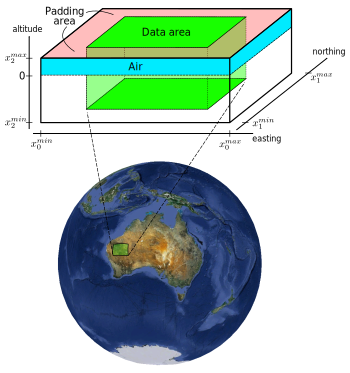
\includegraphics{cartesian}
    \caption{Illustration of domain extents, mapping and padding area}
    \label{fig:cartesianDomain}
\end{figure}

\begin{equation}\label{REF:EQU:INTRO 9}
\begin{array}{rcl}
Q_0  & = &  Q_{\phi} \\
Q_1  & = & -Q_{\theta} \\
Q_2  & = & -Q_r \\
\end{array}
\end{equation}

\section{Sphere Shell Segment}
This is not supported yet.




\section{Driver Classes}
The inversion minimizes an appropriate cost function $J$ to find the physical parameter distribution 
(or more precisely the level set function) which gives the best fit to measured data. A 
particular inversion case (gravity, magnetic or joint) is managed through 
an instance of a specialization of the \class{InversionDriver} class. The task of the class instance
is to set up the appropriate cost function, to manage solution parameters and to run the optimization process.

\subsection{Template}
\begin{classdesc*}{InversionDriver}
template for inversion drivers. By default the limited-memory Broyden-Fletcher-Goldfarb-Shanno (\emph{L-BFGS})~\cite{L-BFGS}\index{L-BFGS} solver is used.
\end{classdesc*}
 
\begin{methoddesc}[InversionDriver]{getCostFunction}{}
returns the cost function of the inversion. This will be an instance of the \class{InversionCostFunction} class, see section~\ref{chapter:ref:inversion cost function}.
Use this method to access or alter attribute or methods of the underlying cost function.
\end{methoddesc}

\begin{methoddesc}[InversionDriver]{getDomain}{}
returns the domain of the inversion as an \escript \class{Domain} object.
\end{methoddesc}

        
\begin{methoddesc}[InversionDriver]{setSolverMaxIterations}{\optional{maxiter=\None}}
set the maximum number of iteration steps for the solver used to minimize the cost function. The default value is 200.
If the maximum number is reached, the iteration will be terminated and the \exception{MinimizerMaxIterReached} is thrown.
\end{methoddesc}

\begin{methoddesc}[InversionDriver]{setSolverTolerance}{\optional{tol=\None} \optional{, atol=\None}}
set the tolerance for the the solver used to minimize the cost function. If \member{tol} is set the iteration is terminated 
if the relative change of the level set function is less or equal \member{tol}. 
 If \member{atol} is set the iteration is terminated 
if the change of the cost function relative to the initial value is less or equal \member{atol}. If both 
tolerances are set both stopping criteria need to be meet. By default \member{tol}=1e-4 and \member{atol}=\None.
\end{methoddesc}

\begin{methoddesc}[InversionDriver]{getLevelSetFunction}{}
returns the level set function as solution of the optimization problem. This method can only be called if the
optimization process as been completed. If the iteration failed the last available approximation of the
solution is returned.
\end{methoddesc}
        
\begin{methoddesc}[InversionDriver]{run}{}
this method run the optimization solver and returns the physical parameter(s) 
from the output of the inversion. Notice that the \method{setup} method must be called before the first call
of \method{run}.
The call can fail as the maximum number is reached in which case
an \exception{MinimizerMaxIterReached} exception is thrown or as there is an incurable break down in the
iteration in which case an \exception{MinimizerIterationIncurableBreakDown} exception is thrown. 
\end{methoddesc}

\subsection{Gravity Inversion Driver}
For examples of usage please see Chapter~\ref{Chp:cook:gravity inversion}.

\begin{classdesc}{GravityInversion}{}
Driver class to perform an inversion of  Gravity (Bouguer) anomaly data. This class
is a sub-class of the \class{InversionDriver} class. The class uses the standard
\class{Regularization} class for a single level set function, see Chapter~\ref{Chp:ref:regularization},
\class{DensityMapping} mapping, see Section~\ref{Chp:ref:mapping density}, and the 
gravity forward model \class{GravityModel}, see Section~\ref{sec:forward gravity}.
\end{classdesc}

\begin{methoddesc}[GravityInversion]{setup}{
domainbuilder
\optional{, rho0=\None}
\optional{, drho=\None}
\optional{, z0=\None}
\optional{, beta=\None}
\optional{, w0=\None}
\optional{, w1=\None}}
sets up the inversion from an instance \member{domainbuilder} of a \class{DomainBuilder}, see Section~\ref{Chp:ref:domain builder}.
Only gravitational data attached to the \member{domainbuilder} are considered in the inversion.
\member{rho0} defines a reference density anomaly (defaults is 0), 
\member{drho} defines a density anomaly (defaults is $2750 \frac{kg}{m^3}$),
\member{z0} defines the depth weighting reference depth (defaults is \None), and
\member{beta} defines the depth weighting exponent (defaults is \None),
see \class{DensityMapping} in Section~\ref{Chp:ref:mapping density}.
\member{w0} and \member{w1} define the weighting factors
$\omega^{(0)}$ and
$\omega^{(1)}$, respectively (see equation~\ref{EQU:REG:1}).
As default \member{w0}=\None and \member{w1}=1 are used.
\end{methoddesc}

\begin{methoddesc}[GravityInversion]{setInitialGuess}{\optional{rho=\None}}
set an initial guess for the density anomaly. As default zero is used.
\end{methoddesc}

\subsection{Magnetic Inversion Driver}
For examples of usage please see Chapter~\ref{Chp:cook:magnetic inversion}.


\begin{classdesc}{MagneticInversion}{}
Driver class to perform an inversion of magnetic anomaly data. This class
is a sub-class of the \class{InversionDriver} class. The class uses the standard
\class{Regularization} class for a single level set function, see Chapter~\ref{Chp:ref:regularization},
\class{SusceptibilityMapping} mapping, see Section~\ref{Chp:ref:mapping susceptibility}, and the linear
magnetic forward model \class{MagneticModel}, see Section~\ref{sec:forward magnetic}.
\end{classdesc}


\begin{methoddesc}[MagneticInversion]{setup}{
domainbuilder
\optional{, k0=\None} 
\optional{, dk=\None} 
\optional{, z0=\None} 
\optional{, beta=\None}
\optional{, w0=\None}
\optional{, w1=\None}}

sets up the inversion from an instance \member{domainbuilder} of a \class{DomainBuilder}, see Section~\ref{Chp:ref:domain builder}.
Only magnetic data attached to the \member{domainbuilder} are considered in the inversion.
\member{k0} defines a reference susceptibility anomaly (defaults is 0), 
\member{dk} defines a susceptibility anomaly scale (defaults is $1$),
\member{z0} defines the depth weighting reference depth (defaults is \None), and
\member{beta} defines the depth weighting exponent (defaults is \None),
see \class{SusceptibilityMapping} in Section~\ref{Chp:ref:mapping susceptibility}.
\member{w0} and \member{w1} define the weighting factors
$\omega^{(0)}$ and
$\omega^{(1)}$, respectively (see equation~\ref{EQU:REG:1}).
As default \member{w0}=\None and \member{w1}=1 are used.
\end{methoddesc}

\begin{methoddesc}[MagneticInversion]{setInitialGuess}{\optional{k=\None}}
set an initial guess for the susceptibility anomaly. As default zero is used.
\end{methoddesc}

\subsection{Gravity and Magnetic Joint Inversion Driver}
For examples of usage please see Chapter~\ref{Chp:cook:joint inversion}.

\begin{classdesc}{JointGravityMagneticInversion}{}
Driver class to perform a joint inversion of  Gravity (Bouguer) and magnetic anomaly data. This class
is a sub-class of the \class{InversionDriver} class. 
The class uses the standard
\class{Regularization} class for a two level set functions with cross-gradient correlation, see Chapter~\ref{Chp:ref:regularization},
\class{DensityMapping} and \class{SusceptibilityMapping} mappings, see Section~\ref{Chp:ref:mapping}, the 
gravity forward model \class{GravityModel}, see Section~\ref{sec:forward gravity}
and the linear
magnetic forward model \class{MagneticModel}, see Section~\ref{sec:forward magnetic}.
\end{classdesc}


\begin{methoddesc}[JointGravityMagneticInversion]{setup}{
domainbuilder
\optional{, rho0=\None}
\optional{, drho=\None}
\optional{, rho_z0=\None}
\optional{, rho_beta=\None}
\optional{, k0=\None}
\optional{, dk=\None}
\optional{, k_z0=\None}
\optional{, k_beta=\None}
\optional{, w0=\None}
\optional{, w1=\None}
\optional{, w_gc=\None}
}
sets up the inversion from an instance \member{domainbuilder} of a \class{DomainBuilder}, see Section~\ref{Chp:ref:domain builder}.
Gravity and magnetic data attached to the \member{domainbuilder} are considered in the inversion.
\member{rho0} defines a reference density anomaly (defaults is 0), 
\member{drho} defines a density anomaly (defaults is $2750 \frac{kg}{m^3}$),
\member{rho_z0} defines the depth weighting reference depth for density (defaults is \None), and
\member{rho_beta} defines the depth weighting exponent for density (defaults is \None),
see \class{DensityMapping} in Section~\ref{Chp:ref:mapping density}.
\member{k0} defines a reference susceptibility anomaly (defaults is 0), 
\member{dk} defines a susceptibility anomaly scale (defaults is $1$),
\member{k_z0} defines the depth weighting reference depth for susceptibility (defaults is \None), and
\member{k_beta} defines the depth weighting exponent for susceptibility (defaults is \None),
see \class{SusceptibilityMapping} in Section~\ref{Chp:ref:mapping susceptibility}.
\member{w0} and \member{w1} define the weighting factors
$\omega^{(0)}$ and
$\omega^{(1)}$, respectively (see equation~\ref{EQU:REG:1}). 
\member{w_gc} sets the weighting factor $\omega^{(c)}$ for the cross gradient term. 
As default \member{w0}=\None, \member{w1}=1 and \member{w_gc}=1 are used.
\end{methoddesc}

\begin{methoddesc}[JointGravityMagneticInversion]{setInitialGuess}{\optional{rho=None, } \optional{k=\None}}
set initial guesses for density and susceptibility anomaly. As default zeros are used.
\end{methoddesc}










 
